\section{Welcome Screens}

\begin{figure}[H]
    \centering
     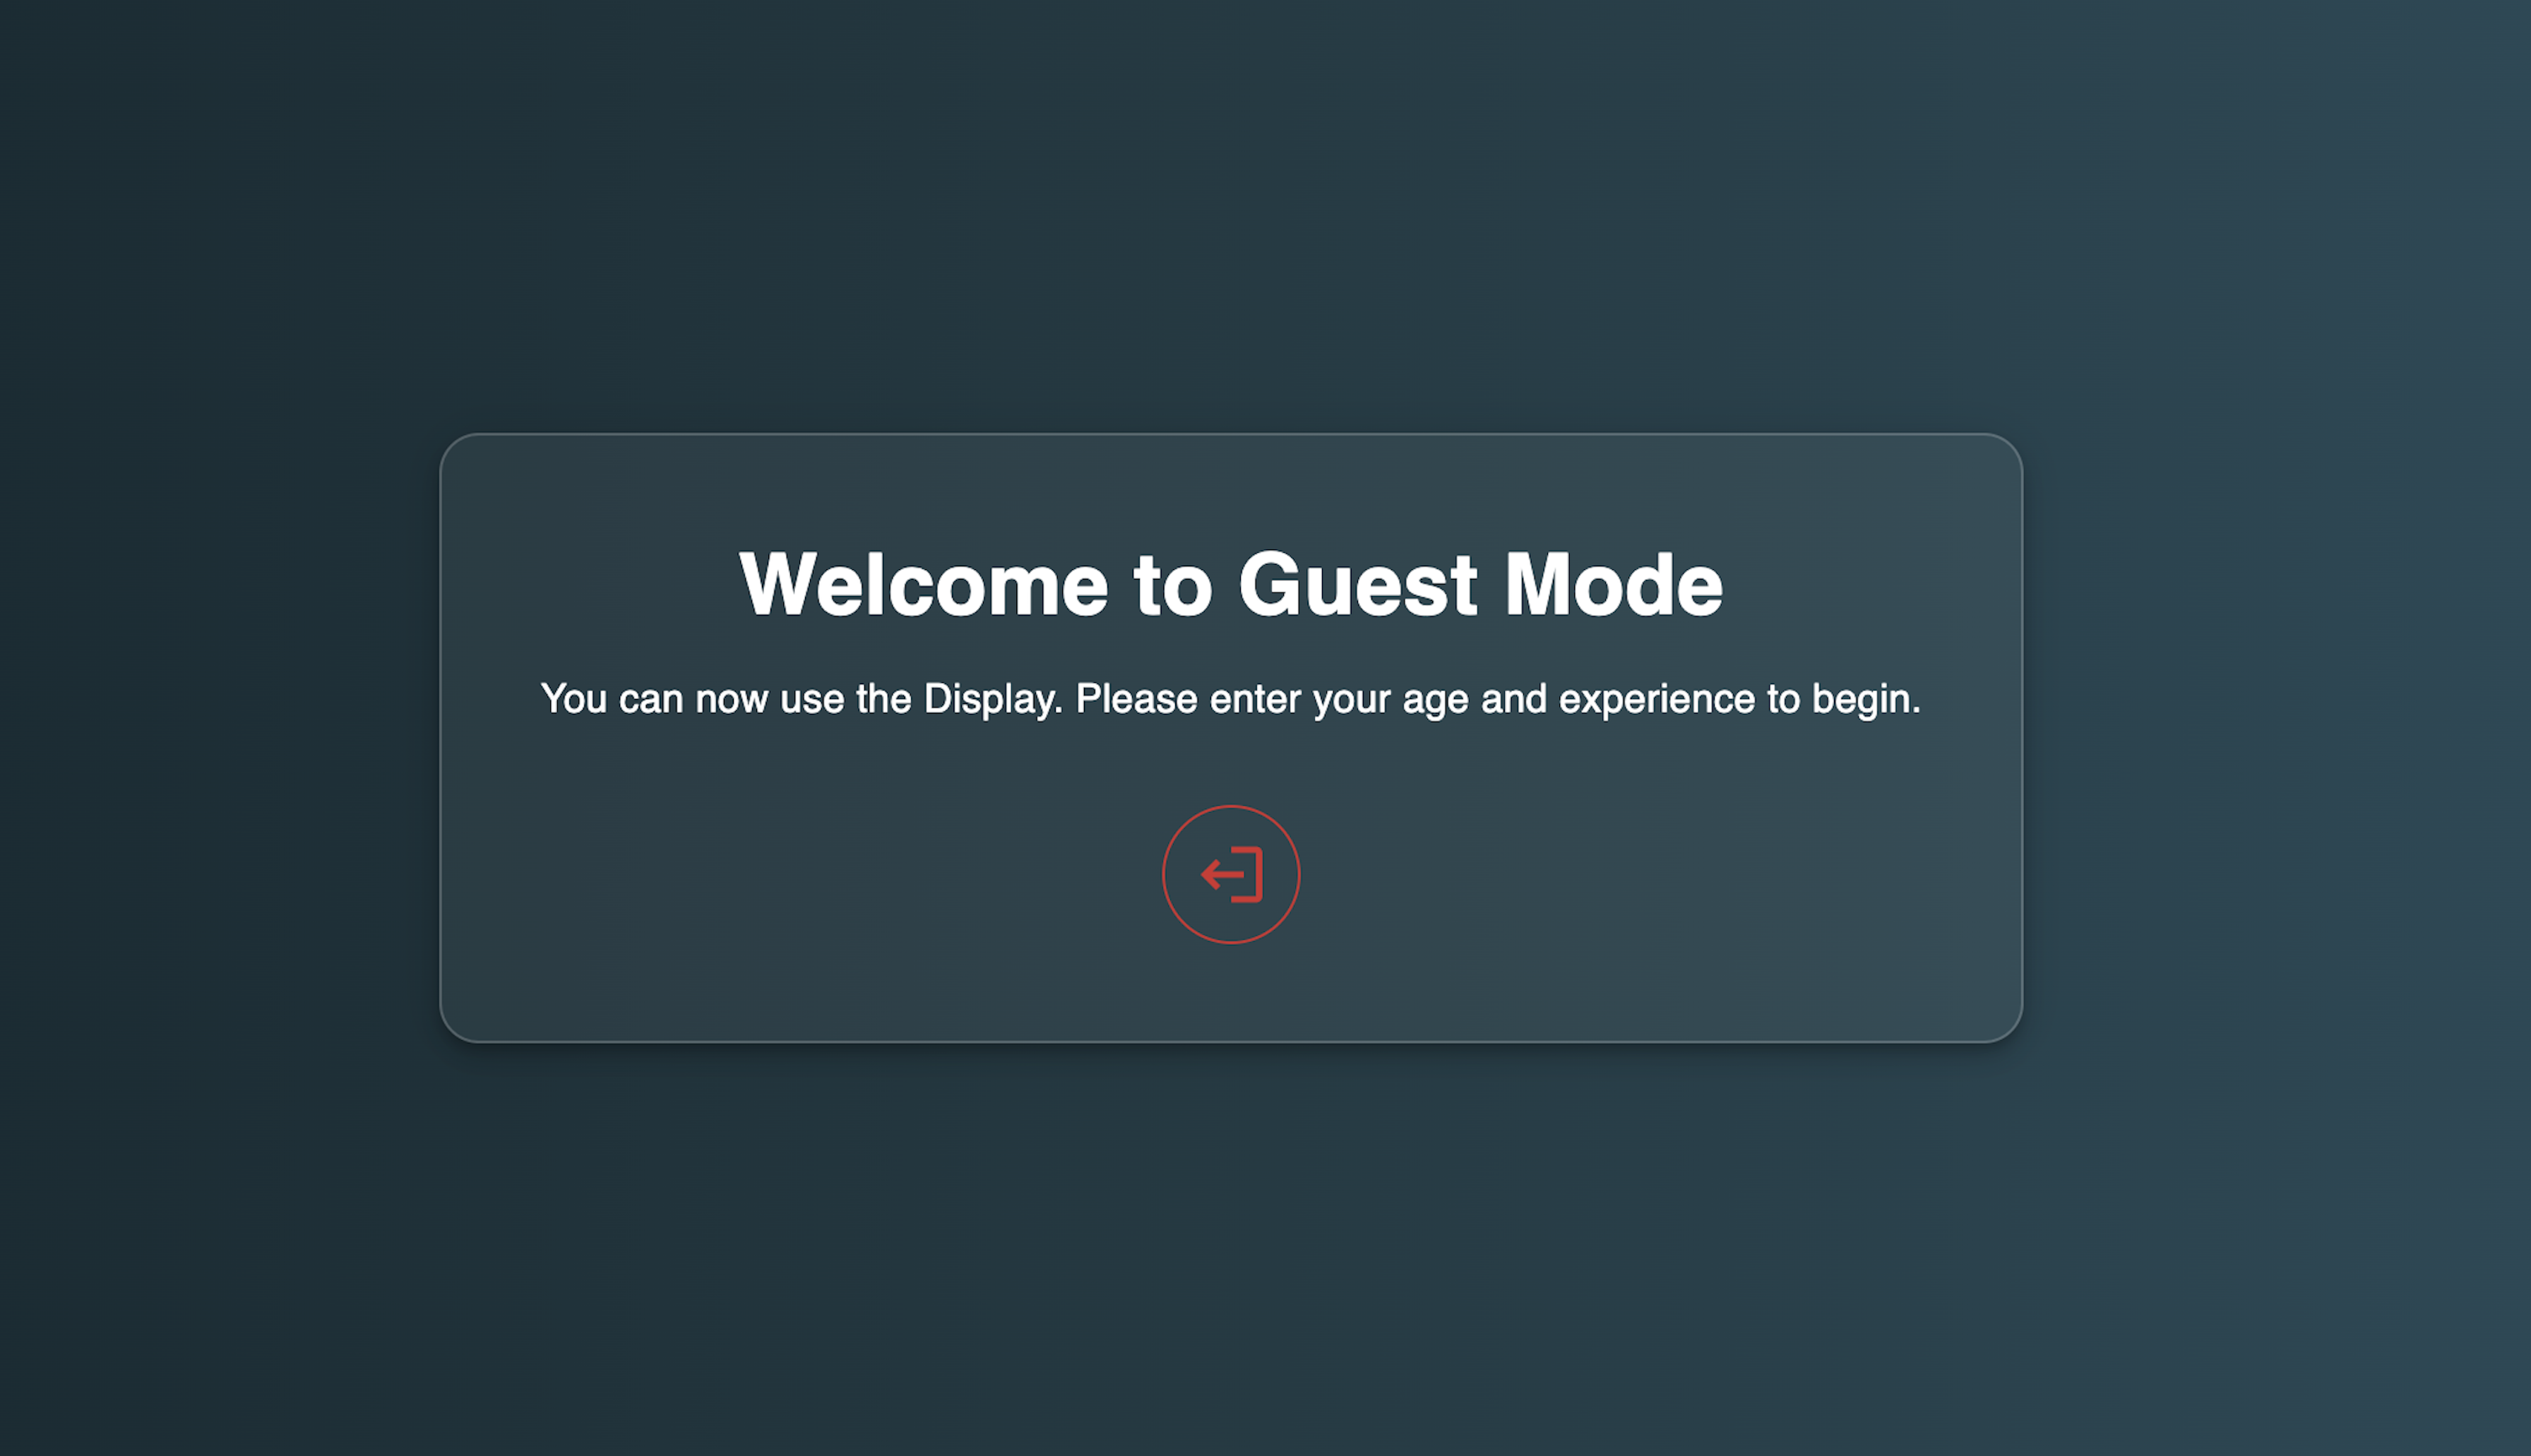
\includegraphics[width=0.6\textwidth]{images/WelcomeScreen.png}
     \caption{Main When connected}
\end{figure}
When the user scans the QR code with their device, a screen will appear allowing them to leave the 
session remotely without needing to interact directly with the public display. While connected, 
a \textbf{session token} linked to the user's device is stored on the server, preventing other 
users from interfering with the session.

\begin{figure}[H]
    \centering
    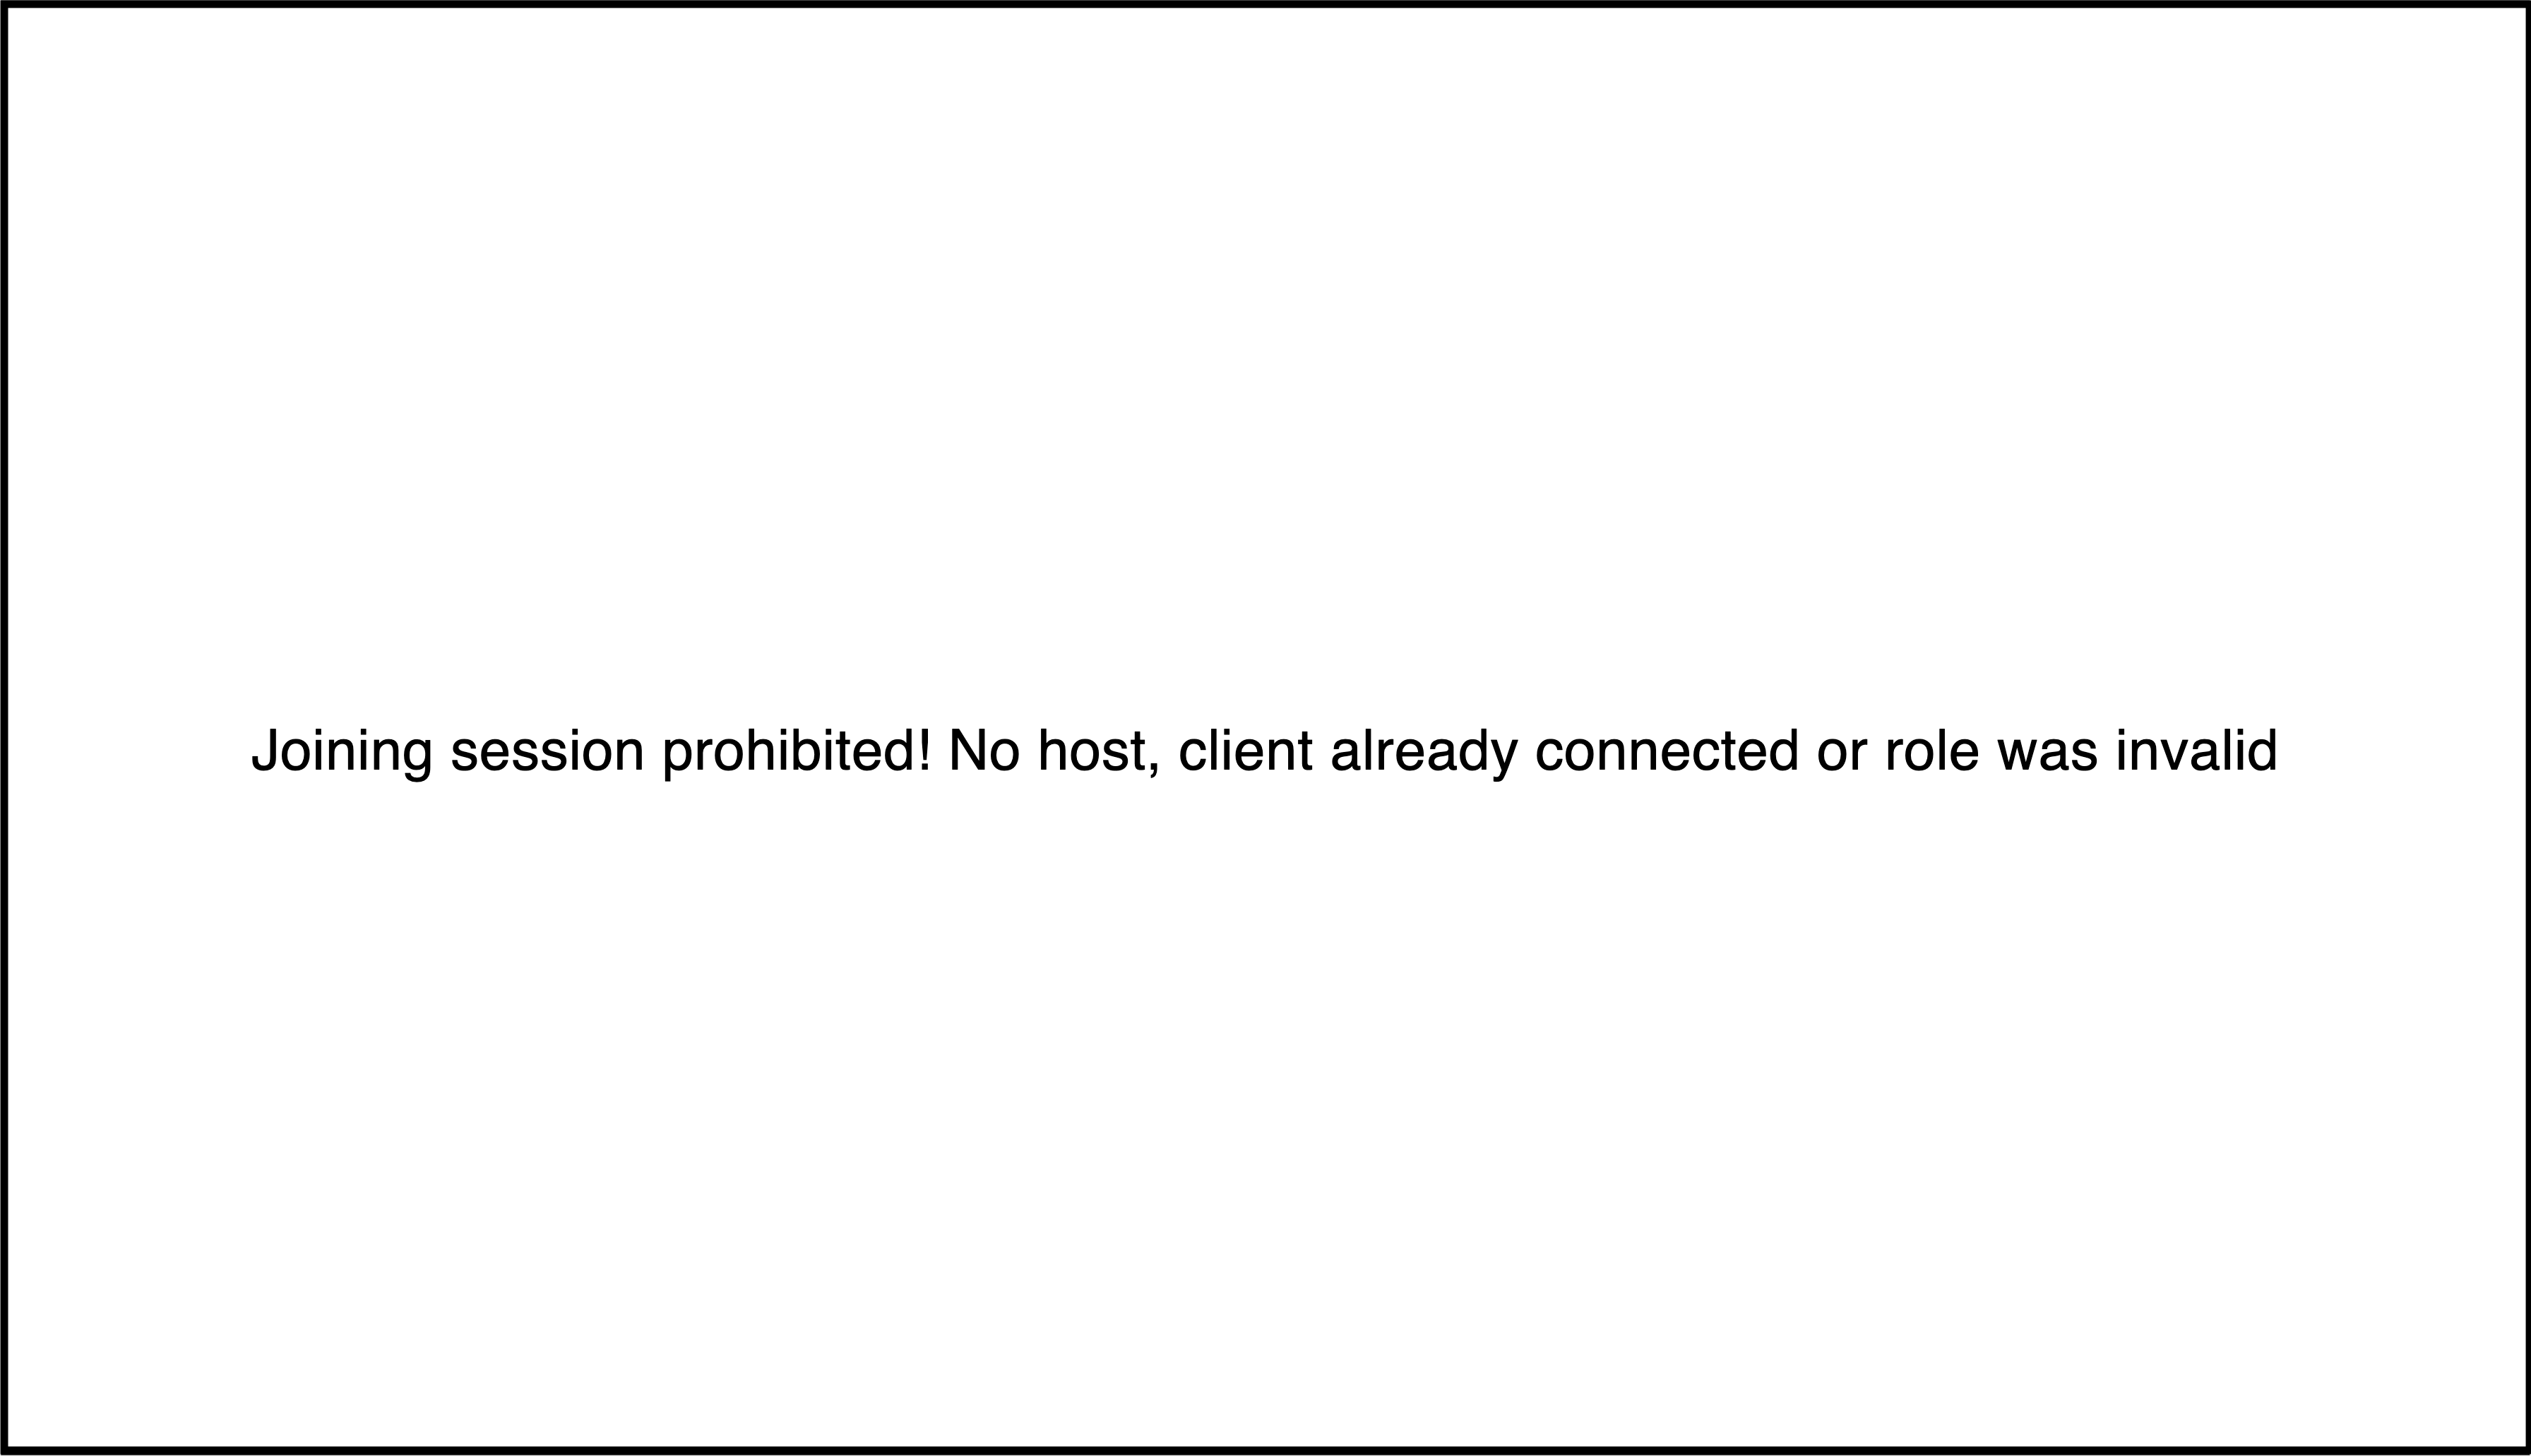
\includegraphics[width=0.6\textwidth]{images/WelcomeScreenInvalid.png}
    \caption{When trying to connect}
\end{figure}
If a user is already connected to the server, any subsequent user who scans the QR code will see 
a different screen on their device, informing them that the \textbf{session is currently occupied}.